% This is LLNCS.DOC the documentation file of
% the LaTeX2e class from Springer-Verlag
% for Lecture Notes in Computer Science, version 2.4
\documentclass{llncs}
\usepackage{llncsdoc}
\usepackage{graphicx}
\usepackage{amssymb}
\usepackage{amsmath}
\usepackage[table]{xcolor}

\usepackage{url}
\urldef{\mailwhajwp}\path|{xxx,yyy,zzz}@mini.pw.edu.pl|
\newcommand{\keywords}[1]{\par\addvspace\baselineskip
\noindent\keywordname\enspace\ignorespaces#1}
%
\begin{document}


\title{Title}
\author{xxx$^{1}$
\and yyy$^1$
\and zzz$^{1}$
}

\authorrunning{xxx}
\institute{$^1$Faculty of Mathematics and Information Science, Warsaw University of Technology\\ul. Koszykowa 75, 00-662 Warsaw, Poland\\
%$^2$Department of Electrical \& Computer Engineering, University of Alberta, \\Edmonton T6R 2G7 AB Canada\\
\mailwhajwp
}

\titlerunning{xxxxx yyyyyy zzzzzz}
\maketitle

\pagestyle{empty}  % no page numbers, no running headers

\begin{abstract}
In the article we present
\end{abstract}


%-------------------------------------------------------------------
%-------------------------------------------------------------------
%-------------------------------------------------------------------

\section{Introduction}
  \label{sec:Introduction}

\textcolor{red} {AJ}
%difference between native and foreign

%why this problem is important

%objectives; what is the contribution of this paper

%novelty elements

%The paper is structured as follows. Section \ref{sec:Literature Review} presents the background knowledge on foreign elements detection present in the literature. Section \ref{sec:preliminaries}


%-------------------------------------------------------------------
%-------------------------------------------------------------------
%-------------------------------------------------------------------
\section{Literature Review}
  \label{sec:Literature Review}
\textcolor{red} {AJ}
%here on 1- outlier detection, 2 - novelty classification, 3 - heavily imbalanced problems, 4 - foreign elements rejection



%-------------------------------------------------------------------
%-------------------------------------------------------------------
%-------------------------------------------------------------------
\section{Preliminaries}
  \label{sec:preliminaries}

%-------------------------------------------------------------------
%-------------------------------------------------------------------
\subsection{The Task of Classification with Rejection}
\textcolor{red} {AJ}
%the task of classification is ...

%...

%-------------------------------------------------------------------
%-------------------------------------------------------------------
\subsection{Regression}
\textcolor{red} {AZ, PW}
% regression, description of variants used in the experiments
Regression analysis is a statistical process for estimating the relationships between variables. It includes many techniques for modeling and analyzing several variables, when the focus is on the relationship between a dependent variable and one or more independent variables. The estimation target is a function of the independent variables called the regression function. There are many different regression models: linear regression, polynomial regression, logistic regression, Bayesian Ridge regression, etc. In this paper we will focus mainly on two regression variants: logistic regression and polynomial one (please note that linear regression is in fact polynomial regression using polynomial of degree 2). \\

Logistic regression relies on the assumption that the independent variables are dichotomous (it means that their values are either 0 or 1), in other words they describe presence or absence of certain facts. In this model, the probabilities describing the possible outcomes of a single trial are modelled using a logistic function. The received answer is evaluated using maximum likelihood method. Predicted values are probabilities and are therefore restricted to (0,1) through the logistic distribution function. \\ % description of logistic regression

Polynomial regression can be viewed as a model that uses linear regression extended by constructing polynomial features from the coefficients. This approach maintains the generally fast performance of linear methods, while allowing them to fit a much wider range of data. The predictors resulting from the polynomial expansion of the "baseline" predictors are known as interaction features, and can be used in classification problem. Just like linear regression, polynomial regression models are usually fit using the method of least squares. \\


% how to perform classification using regression



%-------------------------------------------------------------------
%-------------------------------------------------------------------
\subsection{Rejection Mechanism Based on Regression}
\textcolor{red} {AZ, PW}
%description of the idea of rejection using regression
Calculations presented in this paper were conducted on a mixed set consisting of letters and digits. Because the aim of our work was to provide classifier-based solution for classifying digits and rejecting other symbols, we decided to compare three different approaches towards this problem. All of them based on the assumption that there is no information regarding outliers during classifier training. \\

As the first way to deal with presented issue "one-versus-all" method was prepared. This approach requires creating a vector of classifiers constructed in a specific way. Each classifier has to be trained on a specially prepared training data, consisting of two sets: the first one (denoted as class\_1) holding all training data entries for certain native class, and the second one (denoted as class\_2) being the result of a subset sum operation performed on the rest of the classes except for the class used in class\_1 set. Please note that both class\_1 and class\_2 sets should have the same size, so it is advisable to randomly choose elements when creating class\_2. One classifier for each native class has to be present in a final vector. The actual classification with rejection is performed by presenting the unknown pattern to each of the classifiers from the vector. When the classifier recognizes element as a native one (belonging to class\_1) then the pattern is treated as a recognized, and classified native element. In case of all classifiers rejecting such pattern (classifying it as element from class\_2), it is treated as outlier and rejected. It is also worth noting that there is a possibility of more than one classifier recognizing the pattern as a native element. In such case randomly chosen class is assigned to this pattern. \\

The second approach uses "one-versus-one" method. Similarly to the previous one it requires preparing vector of classifiers, but this time it consists of ${n}\choose{2}$ classifiers, where n is the number of unique native classes. Each classifier is trained on data consisting of two sets: the first one (denoted as class\_1) holding all training data entries for certain native class, and the second one (denoted as class\_2) holding all training data entries for some other class (not the same as class\_1). In the end there is one classifier for each pair of classes: 1 vs. 2, 1 vs. 3, \dots, 1 vs. n, \dots, (n-1) vs. n. Classification with rejection mechanism is based on presenting unknown pattern to every classifier in the vector and remembering their answers (e.g. classifier constructed for 1 vs. n classes can classify pattern as belonging to class 1 or class n). In the end those answers can be presented as a n-wide array with each element being the number of times pattern was classified as belonging to certain class. The pattern is rejected when difference between two biggest values in the result array is smaller than two. In such case it is assumed that classifiers were uncertain as to which class should this unknown element belong to. Otherwise the pattern is classified as an element from the class which had the biggest value in the result array. \textcolor{green}{tutaj można dodać schemat prezentujący opisaną koncepcję} \\\\

The last prepared and examined method, presented in this work, bases on the way of constructing classifiers vector used in the second approach ("one-versus-one"). The difference between those two methods lies in a rejection mechanism. In this method an unknown pattern is treated as a foreign element if its biggest value in the result array is lesser than (n-1). What it actually means is that there must be a certain class that has always been chosen by a classifier from the vector. \textcolor{green}{tutaj można dodać schemat prezentujący opisaną koncepcję} \\




%-------------------------------------------------------------------
%-------------------------------------------------------------------
\subsection{Quality Evaluation}
\textcolor{red} {AJ}
%measures for quality evaluation: precision, recall, ...
\begin{itemize}
\item CC  (Correctly Classified) - the number of correctly classified patterns, i.e. native patterns classified as native ones with the correct class, % and foreign patterns classified as foreign ones,
\item TP  (True Positives) - the number of native patterns classified as native (no matter, into which native class),
\item FN  (False Negatives) - the number of native patterns incorrectly classified as foreign,
\item FP  (False Positives) - the number of foreign patterns incorrectly classified as native,
\item TN  (True Negatives) - the number of foreign patterns correctly classified as foreign.
\end{itemize}


%
%\begin{eqnarray}
%            \textnormal{Accuracy} &\!\!=\!\!& \frac{\textnormal{TP+TN}}{\textnormal{TP+FN+FP+TN}}\nonumber\\\nonumber\\
%     \textnormal{Strict Accuracy} &\!\!=\!\!& \frac{\textnormal{CC+TN}}{\textnormal{TP+FN+FP+TN}}\nonumber\\\nonumber\\
%    \textnormal{Native Precision} &\!\!=\!\!& \frac{\textnormal{TP}}{\textnormal{TP+FP}}\nonumber\\\nonumber\\
%  \textnormal{Native Sensitivity} &\!\!=\!\!& \frac{\textnormal{TP}}{\textnormal{TP+FN}}\nonumber\\\nonumber\\
%  \textnormal{Strict Native Sensitivity} &\!\!=\!\!& \frac{\textnormal{CC}}{\textnormal{TP+FN}}\nonumber\\\nonumber\\
%          \textnormal{Fine Accuracy} &\!\!=\!\!& \frac{\textnormal{CC}}{\textnormal{TP}}\nonumber\\\nonumber\\
%   \textnormal{Foreign Precision} &\!\!=\!\!& \frac{\textnormal{TN}}{\textnormal{TN+FN}}\nonumber\\\nonumber\\
% \textnormal{Foreign Sensitivity} &\!\!=\!\!& \frac{\textnormal{TN}}{\textnormal{TN+FP}}\nonumber\\\nonumber\\
%          \textnormal{F--measure} &\!\!=\!\!& 2\cdot\frac{\textnormal{Precision}\cdot\textnormal{Sensitivity}} {\textnormal{Precision}+\textnormal{Sensitivity}}\nonumber\\\nonumber
%\end{eqnarray}
%
%
%\begin{itemize}
%  \item \emph{Strict Accuracy} is the absolute measure of the classifier's performance. It is the ratio of the number of all \emph{correctly} classified patterns, i.e. native patterns classified to their respective classes and rejected foreign ones to the number of all patterns being processed.
%  \item \emph{Accuracy} is a characteristic derived from strict accuracy by ignoring the need to classify native patterns to their respective classes; in other words, it is sufficient to correctly identify whether a~pattern is native or foreign one. This measure describes the ability to distinguish between native and foreign patterns.
%  \item \emph{Native Precision} is the ratio of the number of not rejected native patterns to the number of all not rejected patterns (i.e. all not rejected native and foreign ones). Native Precision evaluates the ability of the classifier to distinguish native patterns from foreign ones. The higher the value of this measure, the better ability to distinguish foreign elements from native ones. Native Precision does not evaluate how effective identification of native elements is.
%  \item \emph{Native Sensitivity} is the ratio of the number of not rejected native patterns to all native ones. This measure evaluates the ability of the classifier to identify native elements. The higher the value of Native Sensitivity, the more effective identification of native elements. Unlike the Native Precision, this measure does not evaluate the effectiveness of separation between native and foreign elements.
%  \item \emph{Strict Native Sensitivity} takes only correctly classified native patterns and does not consider native patterns, which are not rejected and assigned to incorrect classes, unlike \emph{Native Sensitivity}, where all not rejected native patterns are taken into account.
%  \item \emph{Fine Accuracy} is the ratio of the number of native patterns classified to correct classes, i.e. assigned to their respective classes, to the number of all native patterns not rejected. This measure conveys how precise is correct classification of not rejected patterns.
%  \item \emph{Foreign Precision} corresponds to Native Precision.
%  \item \emph{Foreign Sensitivity} corresponds to Native Sensitivity.
%  \item  Precision and Sensitivity are complementary and there exists yet another characteristic that combines them: the \textit{F--measure}. It is there to express the balance between precision and sensitivity since these two measures affect each other. Increasing sensitivity can cause a~drop in precision since, along with correctly classified elements, there might be more incorrectly classified,
%\end{itemize}

%-------------------------------------------------------------------
%-------------------------------------------------------------------
%-------------------------------------------------------------------
\section{Experiments}
  \label{sec:Experiments}

%-------------------------------------------------------------------
%-------------------------------------------------------------------
\subsection{Presentation of Datasets}
\textcolor{red} {AJ}
\vspace{-3pt}

We present a study on handwritten digits recognition and handwritten letters (from the Latin alphabet) rejection. In other words, native patterns set is made of digits (it is a ten class problem), while foreign patterns are 26 different handwritten letters. The justification to assume such foreign dataset for testing purposes is that appearance of other real-world symbols, but not belonging to any proper class, is a common issue in a~character recognition problem. 

We would like to stress again, that foreign patterns do not participate in the model building phase. The entire scheme is based on native patterns only. Handwritten letters are used only for rejection mechanisms quality evaluation. Samples of processed patterns are displayed in Figure \ref{fig:nativeforeignpatterns}.

The native training dataset consisted of 10,000 handwritten digits with approximately 1,000 observations in each class taken from publicly available MNIST database, \cite{LeCunCortesBurges}. We split each class in proportion ca. 7:3 and as a result we got two sets. The first one includes 6,996 patterns and is used for training. The second set, the test set, contains 3,004 patterns. The dataset of foreign patterns contains 26,383 handwritten Latin letters, ca. 1,000 letters in each class. This dataset was created by 16 students, writing about 70 copies of each letter.

All patterns were normalized and feature vectors comprising of 106 numerical features were created. Examples of features are: maximum/position of maximum values of projections, histograms of projections, transitions, offsets; raw moments, central moments, Euler numbers etc.  The best first search for the optimal feature subset has been performed using FSelector R package, \cite{Romanski} and then analysis of variance was employed to select good features. The final feature vector contained 24 elements. We considered features standardization but the training data is sufficiently consistent (there are no outliers), so we normalized those features to bring linearly all values into the range [0,1]. 


\begin{figure}[!t]
  \centering
  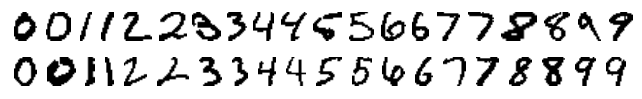
\includegraphics[width=0.49\textwidth]{_Figures/native}
  \caption{...}
\label{fig:nativeforeignpatterns}
\end{figure}


%-------------------------------------------------------------------
%-------------------------------------------------------------------
\subsection{Impact on Classification}
\textcolor{red} {AZ, PW}
%ideally rejection improves classification by rejecting those element that would have been incorrectly classified

\begin{table*}[t]
\centering
\caption{Results for classification without rejection on train and test sets of native patterns in comparison with classification results with rejection mechanism. }
\vspace{3pt}
\setlength{\tabcolsep}{6pt}
\renewcommand{\arraystretch}{1}
\begin{tabular}{|r||cc|cc|}
\hline
& \multicolumn{2}{c|}{no rejection} & \multicolumn{2}{c|}{with rejection}  \\
\hline
&&&&\\
\hline
\end{tabular}
\vspace{12pt}
\label{tab:NativeNoForeign}
\end{table*}


%-------------------------------------------------------------------
%-------------------------------------------------------------------
\subsection{Rejection Quality}
\textcolor{red} {AZ, PW}

The results of our study is presented in Table \ref{tab:NativeNoForeign2}. As it can be seen Polynomial Regression model achieved better accuracy in classifying native patterns and was better at rejecting the foreign ones. It turned out that the third approach (Method 3) yielded the best results whereas the second one performed the worst. Method 2 was the one that "destroyed" classification capabilities of classifiers and had tendency to reject native patterns. On the other hand Method 1 accepted most of the foreign elements. Those results become more obvious if one look at them from the methods' construction point of view. \\

The first approach rejected input only after n failed tests which makes rejection less probable the more tests are performed (more native classes means more tests). Provided pattern was treated as native and labelled as an element from the first class that had its test passed. Because tests were done in order (from class 1 to class n) we observed increased number of classified elements in the first few classes.\\

The second method required certain class to be obviously "stronger" than the others in terms of classification. All patterns that had similarities between two or more different classes were rejected which resulted in poor classification capabilities. \\

The third way provided some sort of equilibrium between classification and rejection by modifying method 2. Elements were rejected only when there was no strong evidence that they belong to certain class. This evidence was in fact the number of times pattern was assigned certain class' label. If there was no class with required number of labels the element was identified as foreign one.

\begin{table}[!b]
	\vspace{-12pt}
	\centering
	\caption{Results for classification with rejection when using only classifiers with three different approaches.}
	\vspace{-6pt}
	\setlength{\tabcolsep}{3pt}
	\renewcommand{\arraystretch}{1}
	{\footnotesize
		\begin{tabular}{|r||c|c|c||c|c|c||c|c|c|}
			\hline
			& \multicolumn{2}{c||}{Method 1} & \multicolumn{2}{c||}{Method 2} & \multicolumn{2}{c|}{Method 3}\\
			\hline
			Regression type & $\;\;$Polynomial$\;\;$ & $\,$Logistic$\;\;$ & $\,$Polynomial$\;\;$ & $\,$Logistic$\;\;$ & $\,$Polynomial$\;\;$ & $\,$Logistic  \\
			\hline
			Data Set & \multicolumn{6}{c|}{Native Patterns, Train Set} \\
			\hline
			Strict Accuracy     & $0.137$ & $0.186$ & $0.716$ & $0.726$ & $0.888$ & $0.236$ \\
			Fine Accuracy       & $0.645$     & $0.731$ & $1$ & $0.897$ & $1$ & $0.926$ \\
			Strict Native Sens. & $0.645$ & $0.720$ & $0.610$ & $0.030$ & $1$ & $0.921$ \\
			\hline
			Data Set & \multicolumn{6}{c|}{Native Patterns, Test Set} \\
			\hline
			Strict Accuracy  & $0.064$ & $0.114$ & $0.719$ & $0.820$ & $0.853$ & $0.143$ \\
			Fine Accuracy       & $0.602$ & $0.738$ & $0.969$ & $0.882$ & $0.959$ & $0.925$ \\
			Strict Native Sens. & $0.601$ & $0.727$ & $0.494$ & $0.030$ & $0.811$ & $0.920$ \\
			\hline
		\end{tabular}
	}
	\vspace{-6pt}
	\label{tab:NativeNoForeign2}
\end{table}


\subsection{Experimental Settings}
\vspace{-3pt}

Solutions presented in this paper have been implemented in Python programming language, using scientific libraries \cite{NumPy,Scikit} and their implementations for logistic and polynomial regression. Several tests have been performed in order to find best suited method parameters for both classifiers. For finding those values the Grid Search~\cite{Scikit} has been used.


%-------------------------------------------------------------------
%-------------------------------------------------------------------
%-------------------------------------------------------------------
\section{Conclusion}
  \label{Conclusion}

\textcolor{red} {AJ}
Proposed ...

In future ...

%-------------------------------------------------------------------
%-------------------------------------------------------------------
%-------------------------------------------------------------------

\section*{Acknowledgment}

\noindent The research is partially supported by the .....

%-------------------------------------------------------------------
%-------------------------------------------------------------------
%-------------------------------------------------------------------
\begin{thebibliography}{1}

\bibitem{HempstalkFrankWitten2008}
Hempstalk, K., Frank, E., Witten, I., \emph{One-class classification by combining density and class probability estimation}, Machine Learning and Knowl. Disc. in Databases, pp. 505-519, 2008.

\bibitem{LeCunCortesBurges}
LeCun, Y., Cortes, C., and Burges, C., \emph{The MNIST database of handwritten digits}, in: http://yann.lecun.com/exdb/mnist.

\bibitem{Romanski}
Romanski, P., Kotthoff, L., \emph{Package FSelector}, http://cran.r-project.org/web/packages/FSelector/FSelector.pdf

\bibitem{NumPy}
http://www.numpy.org/

\bibitem{Scikit}
http://scikit-learn.org/stable/

\end{thebibliography}



\end{document}
